
\chapter{深圳鹏程杯}
\label{chap:pengchengbei}

\begin{example}
  在下图中的钉子板上,用橡皮筋最多可以围出几个正方形?

  \begin{center}
    \begin{tikzpicture}[scale=.5, every node/.style={draw,shape=circle,fill=blue,scale=0.1}]
      \foreach \x in{1,2,3,4}{%
        \foreach \y in{1,2,3,4}{%
          \node(N\x\y) at(\x,\y){};
        }
      }
    \end{tikzpicture}
  \end{center}
\end{example}
\begin{proof}[分类讨论] 算法里的分治思想(Divide and Conquer),先分解成小问题,然后对每个小问题分别求解。
  
  可以围出的正方形共有5种形状,考虑每一种形状的个数,然后求和。

  \vspace{0.5cm}

  \begin{center}
    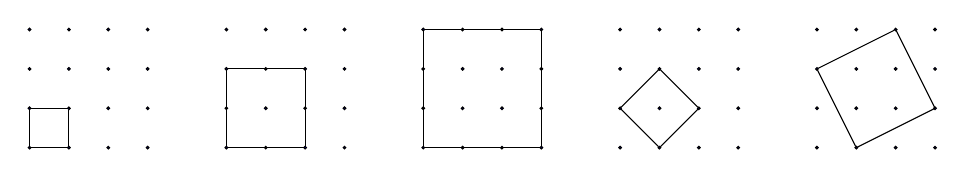
\begin{tikzpicture}[scale=0.5, every node/.style={draw,shape=circle,fill=blue,scale=0.1}]
      \begin{scope}[shift={(0,0)}]
        \foreach \x in{1,2,3,4}{%
          \foreach \y in{1,2,3,4}{%
            \node(N\x\y) at(\x,\y){};
          }
        }
        \draw (N11)--(N12)--(N22)--(N21)--(N11);
      \end{scope}

      \begin{scope}[shift={(5,0)}]
        \foreach \x in{1,2,3,4}{%
          \foreach \y in{1,2,3,4}{%
            \node(N\x\y) at(\x,\y){};
          }
        }
        \draw (N11)--(N13)--(N33)--(N31)--(N11);
      \end{scope}

      \begin{scope}[shift={(10,0)}]
        \foreach \x in{1,2,3,4}{%
          \foreach \y in{1,2,3,4}{%
            \node(N\x\y) at(\x,\y){};
          }
        }
        \draw (N11)--(N14)--(N44)--(N41)--(N11);
      \end{scope}

      \begin{scope}[shift={(15,0)}]
        \foreach \x in{1,2,3,4}{%
          \foreach \y in{1,2,3,4}{%
            \node(N\x\y) at(\x,\y){};
          }
        }
        \draw (N21)--(N32)--(N23)--(N12)--(N21);
      \end{scope}

      \begin{scope}[shift={(20,0)}]
        \foreach \x in{1,2,3,4}{%
          \foreach \y in{1,2,3,4}{%
            \node(N\x\y) at(\x,\y){};
          }
        }
        \draw (N21)--(N42)--(N34)--(N13)--(N21);
      \end{scope}

    \end{tikzpicture}
  \end{center}
\end{proof}


\begin{example}
  一个展厅有120盏灯,分别由编号为1~120的开关控制,这些开关每按一下,对应灯的亮灭状态就会变化一次。开始的时候120盏灯全是熄灭的。老师请大毛把所有编号是2的倍数的开关都按一下,然后又请二毛把所有编号是3的倍数的开关都按一下,然后又请三毛把所有编号是5的倍数的开关都按一下。现在有几盏灯是亮的?
\end{example}

这种题用文氏图表达就很清晰。用三个圆分别表示2的倍数的编号集合,3的倍数的编号集合,5的倍数的编号集合。那么被一个圆覆盖的表示被按了1次,被2个圆覆盖的表示被按了2次,被3个圆覆盖的表示被按了3次。因为开始全是灭的,因此被按了奇数次的开关对应的灯最后是改变了状态变成了亮的,即最终亮着的灯的个数对应于图中阴影部分元素个数。

\begin{center}
  \begin{tikzpicture}[scale=1.0]
    \draw(0,0)--(8,0)--(8,6)--(0,6)--cycle;
    % \draw[fill=blue!30, even odd rule]
    \coordinate[label=2的倍数] (A) at (3,2);
    \coordinate[label=3的倍数] (B) at (5,2);
    \coordinate[label=5的倍数] (C) at (4,4);
    \coordinate[label=$S_{23}$] (D23) at ($0.5*(A)+0.5*(B)$);
    \coordinate[label=$S_{35}$] (D35) at ($0.5*(B)+0.5*(C)$);
    \coordinate[label=$S_{52}$] (D52) at ($0.5*(C)+0.5*(A)$);
    \coordinate[label=$\Delta$] (D235) at ($1/3*(A)+1/3*(B)+1/3*(C)$);

    \fill[blue!30] (A) circle(1.5);
    \fill[blue!30] (B) circle(1.5);
    \fill[blue!30] (C) circle(1.5);
    
    \begin{scope}
      \clip (A) circle(1.5);
      \clip (B) circle(1.5);
      \fill[white] (A) circle(1.5);
    \end{scope}
    \begin{scope}
      \clip (B) circle(1.5);
      \clip (C) circle(1.5);
      \fill[white] (B) circle(1.5);
    \end{scope}
    \begin{scope}
      \clip (C) circle(1.5);
      \clip (A) circle(1.5);
      \fill[white] (C) circle(1.5);
    \end{scope}
    
    \begin{scope}
      \clip (A) circle(1.5);
      \clip (B) circle(1.5);
      \clip (C) circle(1.5);
      \fill[blue!30] (A) circle(1.5);
    \end{scope}

    \draw (A) circle(1.5);
    \draw (B) circle(1.5);
    \draw (C) circle(1.5);

  \end{tikzpicture}
\end{center}


\section{2014}
\label{sec:pengcheng2014}

\begin{example}
  The area of the shadow is 48. What the total area of the 10 circles?
  \begin{center}
    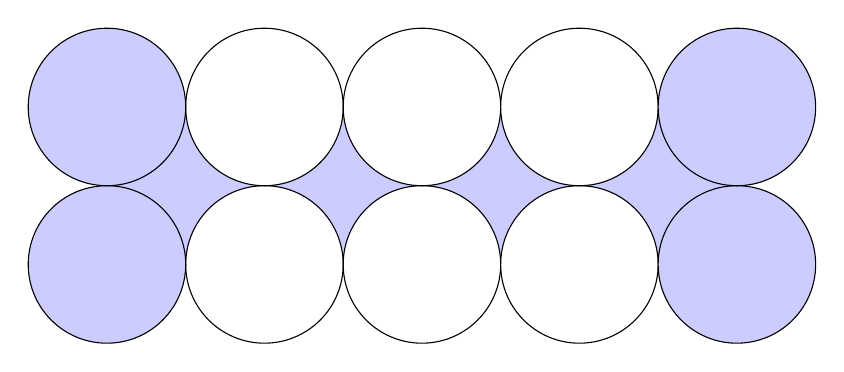
\begin{tikzpicture}[scale=1.0]
      \fill[color=blue!20](0,0)rectangle(8,2);
      \foreach \x/\y in{%
        2/0, 4/0, 6/0,
        2/2, 4/2, 6/2
      }{
        \draw[fill=white](\x,\y) circle(1);
      }        
      \foreach \x/\y in{%
        0/0, 0/2, 8/0, 8/2
      }{
        \draw[fill=blue!20](\x,\y) circle(1);
      }
    \end{tikzpicture}
  \end{center}
\end{example}

The area of the shadow is 4 circles \tikz{\draw[fill=blue!20](0,0)circle(1);} and 4 \tikz{\draw[fill=blue!20](1,0)arc(0:90:1)arc(270:360:1)arc(180:270:1)arc(90:180:1)--cycle;}
% \foreach \x/\y/\s/\t in{1/0/0/90,0/1/270/360,1/2/180/270,2/1/180/270}{\draw[fill=white](\x,\y)arc(\s:\t:1);}}

One circle and one star shape could reshape into a square:
\begin{center}
  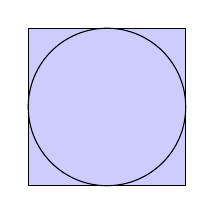
\begin{tikzpicture}
    \draw[fill=blue!20](0,0)rectangle(2,2);
    \draw(1,1)circle(1);
  \end{tikzpicture}
\end{center}

So the area of the square is $48\div4=12$, and the length of each side of the square is $12\div 4=3$, the radius of the circle is $3\div2=\frac32$, the total area of the 10 circles is $10\times \pi\times\left(\frac32\right)^2=10\times\pi\times\frac94=\frac{45\pi}{2}$.


\chapter{Graph}
\label{ch:graph}

\begin{example}
  60 biscuits, 5 kids, some guests. Each kid gives every guest he knows 1 biscuit. And each guest gives every kid he doesn't know 1 biscuit. Exactly 60 biscuits used. How many guests?  
\end{example}

Assumption: KNOW is bi-direction, which means if A knows B, then B must knows A.

偶图(Bipartite graph)
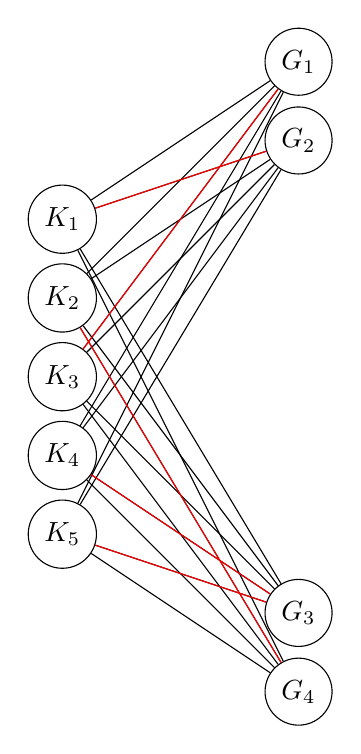
\begin{tikzpicture}[scale=1.0]
  \foreach \y/\n in {5/1,4/2,3/3,2/4,1/5}{%
    \node(K\n)[draw, circle] at(0, \y) {$K_{\n}$};
  }
  \foreach \y/\n in {7/1,6/2,0/3,-1/4}{%
    \node(G\n)[draw, circle] at(3,\y) {$G_{\n}$};
  }
  \foreach \k in {1,2,3,4,5}{%
    \foreach \g in {1,2,3,4}{%
      \draw(K\k)--(G\g);
    }
  }
  % override with some edges where guest hands biscuit to kids
  \draw[color=red](G1)--(K3) (G2)--(K1) (G3)--(K4) (G3)--(K5) (G4)--(K2);
\end{tikzpicture}


\chapter{六年级}
\label{chap:pengcheng-grade6}

\section{2019年}
\label{sec:pengcheng-grade6-2019}

\begin{question}
  $\overline{\text{少年}} + \overline{\text{科技}} + \overline{\text{创新}} + \overline{\text{能力}} = 314$,其中不同的汉字表示不同的非0数字,则分数
  \begin{align*}
    \frac{\text{少} + \text{科} + \text{创} + \text{能}}{\text{年} + \text{技} + \text{新} + \text{力}}
  \end{align*}
  的值是$\blankline$。
\end{question}


\begin{question}
  把一笔奖金分给甲乙两个组,平均每人可得到600元;如果只分给甲级,平均每人可得到1000元;如果只分给乙组,平均每人可得$\blankline$元。
\end{question}


\begin{question}
  把如图所示的6个单位正方形组成的$2\times 3$矩形中,标示出两个角$\alpha$和$\beta$,则$\alpha + \beta$的角度是$\blankline$。

  \begin{center}
    \begin{tikzpicture}[scale=1]
      \coordinate(A1)at(0,2);
      \coordinate(A2)at(0,0);
      \coordinate(O)at(1,0);
      \coordinate(B2)at(2,3);
      \coordinate(B1)at(2,0);
      \draw(0,0)rectangle(2,3) (0,1)--(2,1) (0,2)--(2,2) (1,0)--(1,3) (0,2)--(1,0)--(2,3);
      \draw pic["$\alpha$",<->,angle eccentricity=1.6,draw=orange]{angle=A1--O--A2};
      \draw pic["$\beta$",<->,angle eccentricity=1.6,draw=orange]{angle=B1--O--B2};
    \end{tikzpicture}
  \end{center}
\end{question}


\begin{question}
  从十个数$1,2,3,4,5,6,7,8,9,10$中去掉一个数,使得剩下的九个数可分为两组,且这两组数的乘积相等,则去掉的数是$\blankline$。
\end{question}


\begin{question}
  五个不同的自然数,两两之和依次等于$3,4,5,6,7,8,11,12,13,15$这10个值,则这五个自然数的平均数是$\blankline$。
\end{question}


\begin{question}
  梯形$ABCD$中,$AD\parallel BC$,$\angle ABC=90^\circ$。对角线$AC$和$BD$相交于点$O$,且$AB=6$厘米,$BO=3DO$,三角形$AOD$的面积为3平方厘米。则梯形$ABCD$的周长为$\blankline$厘米。

  \begin{center}
    \begin{tikzpicture}[scale=0.4]
      \coordinate[label=below left:$B$](B)at(0,0);
      \coordinate[label=above left:$A$](A)at(0,6);
      \coordinate[label=above right:$D$](D)at(4,6);
      \coordinate[label=below right:$C$](C)at(12,0);
      \draw(A)--node[midway,left]{6}(B)--(C)--(D)--(A)--(C) (B)--(D);
      \tkzInterLL(A,C)(B,D)\tkzGetPoint{O}\tkzLabelPoints[below](O)
      \fill[color=blue!20](A)--(O)--(D)--cycle;
      \node at($1/3*(A)+1/3*(O)+1/3*(D)$){3};
      \tkzMarkRightAngle[color=blue](A,B,C)
    \end{tikzpicture}
  \end{center}
\end{question}


\begin{question}
  从28个自然数$1,2,\cdots,28$中任取$n$个数,使得其中必有2个数的差是7,则$n$的最小值是$\blankline$。
\end{question}



\begin{question}
  核研所每天按时出车沿规定路线定时到达$A$站,接上同时到达$A$站的专家准时到达核研所。有一天,该专家提前55分钟到达$A$站,因接他的车还没来,他就步行向核研所走去。在途中遇到接他的汽车,立即乘上车,这样比通常提前10分钟到达核研所。则汽车速度是专家步行速度的$\blankline$倍。
\end{question}


\begin{question}
  一个长方体的棱长都是质数,其中相邻的两个表面长方形的面积之和是209平方厘米,则这个长方体的体积是$\blankline$立方厘米。
\end{question}


\begin{question}
  设$a,b,c,d$是1--9之间的四个不同的数字,用这四个数字(不能重复)可以组成很多不同的四位数,小明把所有可能组成的四位数加起来,但他不小心把其中一个四位数多加了一遍,结果为128313,那么正确的结果应该是$\blankline$。
\end{question}


\begin{question}
  计算
  \begin{align*}
    \left( 4\frac79 - 0.8 + 3\frac29 \right) \times
    \left[ \left( 7\frac25 + 2.6 \right) \times 1.25 \right]
  \end{align*}
\end{question}



\section{2020年}
\label{chap:pengcheng-2020}

\begin{question}
  若三个质数$x$,$y$,$z$使得等式$x\times y\times z + 7 = 2020$成立,则$x+y+z=\blankline$.
\end{question}
\begin{proof}[提示]
对$x\times y\times z=2013$做质因式分解。
\end{proof}


\begin{question}
  如图所示,由$O$点引出的6条射线形成的角满足:
  \begin{align*}
    \angle AOB=\angle BOC=\angle COD=\angle DOE=\angle EOF=18^\circ
  \end{align*}
  直线$l$分别交这条射线依次于点$M,G,H,K,L,N$,则图中至少有锐角$\blankline$个。

  \begin{center}
    \begin{tikzpicture}[scale=1.0]
      \coordinate[label=below:$O$](O) at (0,0);
      \coordinate[label=above:$A$](A) at (-0.5,3);
      \coordinate[label=above:$B$](B) at ($(O)!1!-18:(A)$); % rotate A around O by 18 degrees (negative for clockwise)
      \coordinate[label=above:$C$](C) at ($(O)!1!-18:(B)$);
      \coordinate[label=above:$D$](D) at ($(O)!1!-18:(C)$);
      \coordinate[label=above:$E$](E) at ($(O)!1!-18:(D)$);
      \coordinate[label=above:$F$](F) at ($(O)!1!-18:(E)$);

      \coordinate(L1) at (-1,2.8);
      \coordinate(L2) at (3,-0.1);

      \draw(O)--(A) (O)--(B) (O)--(C) (O)--(D) (O)--(E) (O)--(F);

      \draw(L1)--(L2)node[below right]{$l$};

      \tkzInterLL(O,A)(L1,L2)\tkzGetPoint{M}
      \tkzInterLL(O,B)(L1,L2)\tkzGetPoint{G}
      \tkzInterLL(O,C)(L1,L2)\tkzGetPoint{H}
      \tkzInterLL(O,D)(L1,L2)\tkzGetPoint{K}
      \tkzInterLL(O,E)(L1,L2)\tkzGetPoint{L}
      \tkzInterLL(O,F)(L1,L2)\tkzGetPoint{N}
      \tkzLabelPoints[below left](M,G)
      \tkzLabelPoints[below](K,N)
      \tkzLabelPoints[above](H,L)

      \tkzDrawPoints(O,M,G,H,K,L,N)
    \end{tikzpicture}
  \end{center}
\end{question}
\begin{proof}[提示]
  分类讨论。
  \begin{itemize}
  \item 点$O$的锐角有4种:$18^\circ$的,$36^\circ$的,$54^\circ$的,$72^\circ$的。
  \item 直线$l$上的角。每条射线与$l$的夹角,当垂直时没有锐角,当不垂直时有2个锐角。$l$最多只能与其中一条射线垂直,从而最少有5条射线与$l$不垂直,即这些射线与$l$的夹角最少有$5\times2=10$个锐角的夹角。
  \end{itemize}
\end{proof}

\begin{question}
  四个两位数和乘积$\overline{\text{众志}}\times\overline{\text{成城}}\times\overline{\text{防控}}\times\overline{\text{疫情}}$中,相同的汉字表示相同的数字,不同的汉字表示不同的数字,这个乘积数值的结尾最多可连续有$\blankline$个零?
\end{question}

\begin{question}
  边长分别为 8cm 跟 6cm 的两个正方形$ABCD$和$BEFG$如图并排放在了一起,连接$AF$交$BD$于$P$,则四边形$BPEF$的面积是$\blankline$平方厘米。

  \begin{center}
    \begin{tikzpicture}[scale=0.5]
      \coordinate[label=below left :$A$](A) at(0,0);
      \coordinate[label=below      :$B$](B) at(8,0);
      \coordinate[label=above      :$C$](C) at(8,8);
      \coordinate[label=above left :$D$](D) at(0,8);
      \coordinate[label=below right:$E$](E) at(14,0);
      \coordinate[label=above right:$F$](F) at(14,6);
      \coordinate[label=above right:$G$](G) at(8,6);
      \tkzInterLL(A,F)(B,D)\tkzGetPoint{P}\tkzLabelPoints[above](P)
      \fill[color=blue!20](P)--(B)--(E)--(F)--cycle;
      \draw(A)--node[below]{8cm}(B)--(C)--(D)--(A)--(F)--(G) (D)--(B)--node[below]{6cm}(E)--(F);
    \end{tikzpicture}
  \end{center}
\end{question}


\begin{question}
  由$0,1,2,3,4,5,6,7,8,9$这十个数字,每个数字只用一次排出可能的十位数,将这十位数从小到大自左向右排成一行,则从左向右的第6个数是$\blankline$。
\end{question}


\begin{question}
  一杯盐水,第一次加入一定量的水后,盐水的含盐百分比变为15\%;第二次又加入同样多的水,含盐百分比变为12\%;第三次再加入同样多的水,盐水的含盐百分比将变为$\blankline$\%。
\end{question}


\begin{question}
  1--1000000的自然数中,所有的7的倍数的数之和等于$\blankline$?
\end{question}
\begin{proof}[提示]
  本质是 $7,14,21,\cdots$ 这样一个等差数列求和。
\end{proof}


\begin{question}
  今年,祖父的的年龄是小学生明明年龄的6倍,几年过去了,祖父的年龄将是明明年龄的5倍,又过去了几年以后,祖父的年龄是明明年龄的4倍,祖父今年是$\blankline$岁?
\end{question}
\begin{proof}[提示]
  寻找不变量。随着时间的变化,祖父和明明的年龄差是永远不变的。
  \begin{itemize}
  \item 6倍的时候,年龄差是明明年龄的5倍。
  \item 5倍的时候,年龄差是明明年龄的4倍。
  \item 4倍的时候,年龄差是明明年龄的3倍。
  \end{itemize}
  也就是年龄差是5,4,3的倍数,年龄差是$60,120,180,\cdots$。一般来说,在这个数列里,60是较为合理的爷孙年龄差。故今年,年龄差60是明明年龄的5倍,明明今年是$60\div5=12$岁,祖父今年是$12\times6=72$岁。
\end{proof}


\begin{question}
  如图是一个容积为30立方厘米的正方体铁皮盒被剪去一个“角”后的平面展开图(图中相同字母表示长度相等的线段)各侧面剪掉的三个阴影三角形的面积分别是2平方厘米,3平方厘米,3平方厘米,则该铁皮盒最多可以装$\blankline$立方厘米的水。

  \begin{center}
    \begin{tikzpicture}[scale=2.0]
      \draw(0,0)--++(1,0)--++(0,1)--++(2,0)--++(0,1)--++(-2,0)--++(0,1)--++(-1,0)--++(0,-1)--++(-1,0)--++(0,-1)--++(1,0)--cycle;
      \draw[dashed](0,1)rectangle(1,2) (2,1)--++(0,1);
      \coordinate(A0)at(-1,1);
      \coordinate(A1)at(-1,1.4);
      \coordinate(A2)at(-0.4,1);
      \coordinate(B0)at(0,0);
      \coordinate(B1)at(0,0.6);
      \coordinate(B2)at(0.4,0);
      \coordinate(C0)at(3,1);
      \coordinate(C1)at(2.6,1);
      \coordinate(C2)at(3,1.4);
      \foreach \a/\b/\c in{A0/A1/A2,B0/B1/B2,C0/C1/C2}{
        \draw(\b)--(\c);
        \fill[color=blue!20](\a)--(\b)--(\c)--cycle;
      }
      % Av --> A vertical, Ah --> A horizontal
      \coordinate[label=left:$a$](FAv)at($0.5*(A0)+0.5*(A1)$);
      \coordinate[label=below:$b$](FAh)at($0.5*(A0)+0.5*(A2)$);
      \coordinate[label=left:$b$](FBv)at($0.5*(B0)+0.5*(B1)$);
      \coordinate[label=below:$c$](FBh)at($0.5*(B0)+0.5*(B2)$);
      \coordinate[label=below:$c$](FCv)at($0.5*(C0)+0.5*(C1)$);
      \coordinate[label=right:$a$](FCh)at($0.5*(C0)+0.5*(C2)$);
    \end{tikzpicture}
  \end{center}
\end{question}
\begin{proof}[提示]
  用方程组很方便。三个阴影部分面积分别是$2,3,3$,不妨设
  \begin{align*}
    \begin{cases}
      \frac12\times ab=2\\
      \frac12\times bc=3\\
      \frac12\times ca=3
    \end{cases}
  \end{align*}
  从而$a\times b\times c=12$且$a,b,c$是$2,2,3$的组合,对应的被剪掉部分的体积是
  \begin{align*}
    \frac13 \times \frac12 \times abc=2
  \end{align*}
\end{proof}


\begin{question}
  在2名六年级选手与至少10名五年级选手一起进行比赛象棋,每两个人彼此都恰好比赛一场,每场比赛胜者得2分,负者得0分,若和局则各得到1分。比赛结束后,已知2名六年级的选手得分之和是20分,且每名五年级选手都得到了$N$分,则$N=\blankline$。
\end{question}


\begin{question}
  \begin{align*}
    \left( 5\frac59 - 0.8 + 2\frac49 \right) \times
    \left( 7.6\div\frac45 + 2\frac25 \times 1.25 \right)
  \end{align*}
\end{question}


\begin{question}
  一个六位数$\overline{abcdef}$满足$\overline{defabc}=6\times\overline{abcdef}$,试确定这个六位数$\overline{abcdef}$的值,并且写出求解过程。
\end{question}
\begin{proof}[提示]
  如果想到了$1/7$,那就容易联想。

  想不到,就只能中规中矩。考察$\overline{abcdef}$和$\overline{defabc}$,其实本质只有两部分$\overline{abc}$和$\overline{def}$。从而
  \begin{align*}
    &6\times\overline{abcdef}=\overline{defabc}\\
    \iff & 6\times\left(1000\times\overline{abc} + \overline{def}\right)
           = 1000\times\overline{def} + \overline{abc}\\
    \iff & 857\times\overline{abc}= 142\times\overline{def}
  \end{align*}
  由857与142互质可知三位数$\overline{abc}$和$\overline{def}$分别是142与857。怎么判断两个整数互质?可以用欧拉辗转相除法求其公约数。
\end{proof}


\begin{theorem}[欧拉辗转相除法]
  记$\gcd(a,b)$表示两个整数$a,b$的最大公约数,若$r=a\pmod b$,则有$\gcd(a,b)=\gcd(r,b)$。
\end{theorem}
\begin{example}
求857与142的最大公约数。把大的记为$a$,小的记为$b$,这样余数$r$与$b$的组合才会比$a,b$的组合小,迭代下去总有结束的时候。
\begin{align*}
  847 \pmod{142} = 137 & \implies \,\, \gcd(847,142) = \gcd(137,142) = \gcd(142,137) \\
  142 \pmod{137}= 5   & \implies \,\, \gcd(142,137) = \gcd(5,137)
\end{align*}
由这里已经容易知道5和137是互质的,从而$\gcd(5,137)=1$。若还猜不出来,可以继续下去
\begin{align*}
  137 \pmod 5 = 2 & \implies \,\, \gcd(5,137) = \gcd(2,5) = \gcd(5,2) \\
  5 \pmod 2 = 1   & \implies \,\, \gcd(5,2) = \gcd(1,2)
\end{align*}
这下总是能看出来$\gcd(1,2)=1$了。
\end{example}


\begin{question}
  如图所示,$ABCD$是正方形,$PCD$是面积为1的正三角形,线段$AP$交$BD, CD$分别于$E$跟$L$,$BP$交$CD$于点$K$,取$AB$中点$M$,连接$MK,ML$。
  \begin{enumerate}
  \item 证明:$BE=PE$。
  \item 求四边形$PKML$的面积。
  \end{enumerate}

  \begin{center}
    \begin{tikzpicture}[scale=4.0]
      \coordinate[label=below left :$A$](A)at(0,0);
      \coordinate[label=above left :$B$](B)at(0,1);
      \coordinate[label=above right:$C$](C)at(1,1);
      \coordinate[label=below right:$D$](D)at(1,0);
      \coordinate[label=      left :$M$](M)at($0.5*(A)+0.5*(B)$);
      \coordinate[label=right      :$P$](P)at($(C)!1!60:(D)$);
      \coordinate[label=above right:$K$](K)at($0.75*(C)+0.25*(D)$);
      \coordinate[label=below right:$L$](L)at($0.25*(C)+0.75*(D)$);
      \tkzInterLL(B,D)(A,P)\tkzGetPoint{E}\tkzLabelPoints[below](E)
      \draw(A)--(B)--(C)--(D)--(A)--(P)--(B) (C)--(P)--(D) (B)--(D) (K)--(M)--(L);
    \end{tikzpicture}
  \end{center}
\end{question}


\begin{question}
  如果一个三角形的三条边长是彼此不等的三个质数,这样的三角形叫做“鹏程三角形”。
  \begin{enumerate}
  \item 试举一个鹏程三角形的实例。
  \item 证明:不存在周长为2020的鹏程三角形。
  \item 证明:鹏程三角形一定不是直角三角形。
  \end{enumerate}
\end{question}


\begin{question}
  在一个平地上站着$n$个人,对每个人来说,他到其他的人的距离均不相同,当有火灾信号发出的时候,每人都用水枪击中距离他最近的人。
  \begin{enumerate}
  \item 当$n=2020$时,请你举例说明,可能每个人都是湿的。
  \item 当$n=2021$时,证明至少有一个人身上是干的。
  \end{enumerate}
\end{question}






\section{Using mind maps to find the way out}
\label{sec:mind-map}

\subsection{Forward mind map}
\label{sec:mind-map-forward}

\subsection{Backward mind map}
\label{sec:mind-map-backward}




